\documentclass[11pt]{beamer}

\usepackage[T1]{fontenc}
% \usepackage{lmodern}

% \usepackage{mathptmx}
% \usepackage{helvet}
% \renewcommand{\rmdefault}{ptm}



\usepackage[final]{listings}
\usepackage{verbatim}
\usepackage{xcolor}
\usepackage{multirow}
\usepackage{multicol}
\usepackage{pgfplots}
\usepackage[normalem]{ulem}
\usepackage[english]{babel}
\usepackage{times}
\usepackage{tikz}
% \usepackage{tabularx}

% --- Setttings
\graphicspath{{figs/}}

% --- Listings
\lstset{escapeinside={(*@}{@*)}}
\lstdefinestyle{lara}{language=C++,
  frame=single, frameround=tttt,
  rulecolor=\color{lightgray},
  morekeywords={aspectdef, var, apply, select, condition, begin, end, input, entry, exit}}
\lstdefinestyle{MaxC}{language=C++,
  morekeywords={s_int32, int32, float8_24, sin_float8_24,
    sout_float8_24, float8_24, s_int, s_float8_24, s_bool, count, countChain,
    CURRENT_CYCLE, MAX_CYCLE, pragma},
  deletekeywords={static}}
\lstdefinestyle{MaxJ}{
  morekeywords={HWVar, io, hwFloat, stream}
}

\lstset{
  basicstyle=\footnotesize,
  keywordstyle=\color{black}\bfseries,
  captionpos=b,
  breaklines=true,
  showspaces=false,
  escapeinside={(*@}{@*)}
}

% --- PGF Plots ---
\pgfplotsset{
  width=0.9\textwidth,
  enlargelimits=0.1,
  compat=1.8,
  tick label style={font=\tiny},
  label style={font=\footnotesize},
  legend style={font=\scriptsize},
  axis line style={lightgray},
}


% --- Tables ---
\renewcommand{\arraystretch}{1.5}


\newcommand{\MAXC}[0]{FAST}
\newcommand\reduline{\bgroup\markoverwith
  {\textcolor{red}{\rule[-0.5ex]{2pt}{0.4pt}}}\ULon}

\mode<presentation>
{
  % \usetheme{Darmstadt}
  % \usetheme{Rochester}
  % \usetheme{Pittsburgh}
  % \usetheme{Singapore}
  % \usecolortheme{whale}
  % \usecolortheme{default}
  % \setbeamercovered{transparent}
  % or whatever (possibly just delete it)
}


% \useinnertheme[]{rounded}
% \useoutertheme{shadow}
% \usecolortheme{orchid}
% \usecolortheme{whale}

\usetikzlibrary{shapes,arrows}

\pgfdeclareimage[height=0.25cm]{tick-green}{images/tick-green.png}
\pgfdeclareimage[height=0.25cm]{tick-gray}{images/tick-gray.png}
\pgfdeclareimage[height=0.3cm]{good}{images/good.png}
\pgfdeclareimage[height=0.3cm]{bad}{images/bad.png}
\pgfdeclareimage[height=0.3cm]{problem}{images/problem.png}
\pgfdeclareimage[height=0.3cm]{idea}{images/idea.png}
\pgfdeclareimage[height=0.3cm]{qm}{images/qm.png}

\definecolor{UniBlue}{RGB}{83,121,190}
\setbeamercolor{title}{fg=UniBlue}
\setbeamercolor{frametitle}{fg=UniBlue}
\setbeamercolor{structure}{fg=UniBlue}

\setbeamertemplate{navigation symbols}{}%remove navigation symb
% \setbeamertemplate{footline}{}
\setbeamertemplate{headline}{}
% \setbeamertemplate{caption}{\figurename}
\setbeamertemplate{footline}[frame number]

\newcommand{\tickgray}{\pgfuseimage{tick-gray}}
\newcommand{\tickgreen}{\pgfuseimage{tick-green}}
\newcommand{\imggood}{\pgfuseimage{good}}
\newcommand{\imgbad}{\pgfuseimage{bad}}
\newcommand{\imgproblem}{\pgfuseimage{problem}}
\newcommand{\imgidea}{\pgfuseimage{idea}}
\newcommand{\imgqm}{\pgfuseimage{qm}}

\title{\Large Aspect Oriented Design for Dataflow Engines}
\author{
  {\small Paul Grigora\c{s}} \\[0.2cm]
  \href{mailto:paul.grigoras09@imperial.ac.uk}{\texttt{\scriptsize paul.grigoras09@imperial.ac.uk}}}
\date{}

\begin{document}

\begin{frame}
  \titlepage
\end{frame}

\section{Introduction}
 \begin{frame}


      \frametitle{Introduction}
      %------------------------------------------------------------ 1
      \only<1>{
        \framesubtitle{Overview}

      }

      \only<2>{
        \framesubtitle{Motivation}
      }

      \only<3>{
        \framesubtitle{Challenges}
      }

      \only<4>{
        \framesubtitle{Contributions
}
      }
  \end{frame}

\section{Desgin Flow}
\begin{frame}{Design Flow}
  \vspace{-0.3cm}
  \begin{figure}
    \centering
    \def\svgwidth{0.88\textwidth}
    \input{figs/asap13-design-flow.pdf_tex}
  \end{figure}
\end{frame}
\section{FAST}

\begin{frame}[fragile]
  \frametitle{2. FAST -- Facile Aspect-driven Source Transformation}

\begin{lstlisting}[style=MaxC]
// kernel defines input, output streams and scalars
void kernel_MovingAvg(float* in, float* avg, int bound)
{
  // special macros implemented as counters
  bool hasPrev = CURRENT_CYCLE >=bound;
  bool hasNext = CURRENT_CYCLE < MAX_CYCLE - bound;
  bool hasBoth = hasPrevious & hasNext;

  // ternary operator, stream offsets, arithmetic
  float prev = hasPrev ? in[-1] : 0.0;
  float next = hasNext ? in[ 1] : 0.0;
  float sum  = prev + in[0] + next;

  // output assignment
  avg[0] = hasBoth? sum / 3 : sum / 2;
}

int main() {
  #pragma fast hw:MovingAvg  // maps to dataflow kernel
  MovingAvg_CPU(...);        // call regular C function
}
\end{lstlisting}
\end{frame}

\begin{frame}
  \frametitle{2. FAST: Features}

\begin{table}[!h]
  \centering
\renewcommand{\arraystretch}{1.4}
\begin{tabular}{l|l|l}
\hline
\bf{Feature}                        & \bf{Description}              & \bf{Method}          \\
\hline\hline
  I/O                               & Kernel arguments              & Inferred             \\
\hline
  Control                           & Ternary op. (?:), \texttt{if} & C99                  \\
\hline
\multirow{2}{*}{Computation}        & +, *, /, -                    & C99                  \\
                                    & log, exp, sqrt, sin etc.      & $<$math.h$>$         \\
\hline
  \multirow{2}{*}{Streams}          & Declared as pointers          & \multirow{2}{*}{C99} \\
                                    & Array index access     &                      \\
\hline
  Optimisation                      & \multirow{2}{*}{C pragmas}    & \multirow{2}{*}{C99} \\
  Hardware \  Mapping               &                               &                      \\
\hline
  \multirow{2}{*}{Parameterization} & Constants, variables,         & \multirow{2}{*}{C99} \\
                                    & \texttt{for}, \texttt{while}  &                      \\
\end{tabular}
\end{table}
\end{frame}

\begin{frame}{2. FAST: FAST vs C}
\begin{itemize}
\item Fast only uses C \emph{syntax}
\begin{itemize}
\item to simplify integration with compilation tools (aspect weaving,
  dataflow, compiler frameworks)
  \item to express dataflow designs in a simple, intuitive fashion
\end{itemize}
\vspace{0.5cm}
\item  Differences compared to C
\begin{itemize}
\item execution model only supports kernels
\item pointers are regarded as   streams
\item negative offsets are allowed
\item only compile time loop bounds are allowed
\item direct interoperability with C code is not possible, but
  simulated via pragmas
\end{itemize}
\end{itemize}

\end{frame}
\section{Aspect Descriptions}
\begin{frame}
  \frametitle{3. Aspect Descriptions}
  \begin{enumerate}
    \setlength{\itemsep}{15pt}
  \item \textbf{System Aspect Descriptions}
    \begin{itemize}
    \item FAST + C application
    \end{itemize}
  \item \textbf{Implementation Aspect Descriptions}
    \begin{itemize}
    \item FPGA and dataflow specific optimisations
    \end{itemize}
  \item \textbf{Exploration Aspect Descriptions}
    \begin{itemize}
    \item user guided design space exploration strategies
    \end{itemize}
  \item \textbf{Development Aspect Descriptions}
    \begin{itemize}
    \item automate repetitive, error-prone development tasks
    \end{itemize}
  \end{enumerate}
\end{frame}

\begin{frame}{System Aspects: Run-time Reconfiguration}
  \begin{itemize}
  \item idle functions may appear in large designs
  \item use run-time reconfiguration to remove idle functions
    \begin{columns}
      \begin{column}{.55\textwidth}
  \begin{figure}[!ht]
    \centering
    \def\svgwidth{\linewidth}
    \input{figs/rtm-desc.pdf_tex}
  \end{figure}
      \end{column}
      \begin{column}{.45\textwidth}
  \begin{figure}[!ht]
    \centering
    \def\svgwidth{\linewidth}
    \input{figs/rtm-idle.pdf_tex}
  \end{figure}
      \end{column}
    \end{columns}


  \end{itemize}
\end{frame}

\begin{frame}[fragile]{System Aspects: Run-time Reconfiguration}
  \begin{itemize}
    \setlength{\itemsep}{8pt}
  \item pragmas specify configuration parameters
\end{itemize}
    \begin{columns}
      \begin{column}{.7\textwidth}
        \begin{center}
          \begin{lstlisting}[style=MaxC]
#pragma fast hw:f1 cfg:c0(Par=2)
x = f(0);
#pragma fast hw:f1 cfg:c1(Par=1)
y = f(x);
#pragma fast hw:g1 cfg:c1(Par=1)
z = g(x, y);
          \end{lstlisting}
        \end{center}
      \end{column}
      \begin{column}{.3\textwidth}
        {\footnotesize
          \begin{table}[!h]
            \renewcommand{\arraystretch}{1.3}
            \hspace{-2cm}
            \begin{tabular}{c|c|c}
              \multicolumn{3}{c}{\bf{partition}} \\
              \hline
              \bf{call.key} & \bf{hw} & \bf{cfg}  \\
              \hline
              main:f:1 & fast\_f0 & c0 \\
              main:f:2 & fast\_f1 & c1 \\
              main:g:3 & fast\_g & c1 \\
            \end{tabular}
          \end{table}
        }
      \end{column}
    \end{columns}

\end{frame}

\begin{frame}[fragile]{3. Aspect Descriptions}
  \frametitle{ System Aspects: Run-time Reconfiguration}
  Map function calls (on the CPU side) to configurations:
  \begin{itemize}
  \item inspect each function call
  \item if part of a partition, add corresponding FAST pragma
  \item $ \text{partition} : \text{funcCall} \rightarrow (\text{kernel}, \text{config}) $
  \end{itemize}

  \begin{lstlisting}[style=lara]
aspectdef AspReconfig
  input: partition
  function.call:
    if (call.key in partition) {
     p = partition[call.key]
     config = p.cfg + '(Par = ' + p.par + ')'
     kernel = p.par
     call.prepend('#pragma fast hw:'kernel' cfg:'config)
    }
end
  \end{lstlisting}
\end{frame}


\begin{frame}[fragile]{3. Aspect Descriptions}
  \frametitle{Implementation Aspects: Operator Optimisation}
  Map computation to Digital Signal Processors:
  \begin{itemize}
  \item $ \text{opMapping} : \overrightarrow{\text{opOccurence}} \rightarrow \text{factor}$
  \item $\text{factor} \in \{\text{none}, \text{balanced}, \text{full}\} $
  \item mapping can be varied by different aspect to support design
    space exploration
  \end{itemize}
  \begin{lstlisting}[label=lst:label, style=lara]
aspectdef DspBalancing
input: opMapping
 function.stmt:
   opUsage = countOperatorUsage(stmt)
   factor  = opMapping[opUsage]
   if (factor != '')
     stmt.prepend('#pragma fast balanceDSP:' + factor);
end
  \end{lstlisting}
\end{frame}

\begin{frame}{3. Implementation Aspects: Operator Optimisation}
  \begin{figure}[!ht]
    \centering
    \def\svgwidth{\linewidth}
    \input{figs/opt-split.pdf_tex}
  \end{figure}

\end{frame}

\begin{frame}[fragile]{3. Aspect Descriptions}
  \frametitle{Exploration Aspect Descriptions: Iterative Exploration}
  Automate design space exploration
  \begin{itemize}
  \item vary an attribute of a dataflow configuration
  \item generate FAST configuration and compile FPGA bitstream
  \item extract feedback from compilation report
  \item stop when a resource usage limit is reached
  \end{itemize}
  \begin{lstlisting}[label=lst:label, style=lara]
aspectdef DesignExploration
input: attribute, start, step, res, res_limit, config
  config[attribute] = start
  do {
    var designName = genName(config)
    generateFASTDesign(designName, config)
    buildFASTDesign(designName)
    config[attribute] += step
  } while (@hw[designName].res < res_limit)
end
  \end{lstlisting}
\end{frame}

\begin{frame}[fragile]{Monitoring and Logging}
  \begin{itemize}
  \item Logging: useful for debugging (no run-time support)
  \end{itemize}
  \begin{lstlisting}[label=lst:label, style=lara]
aspectdef WatchVar
function.vref{is_written}:
  vref.parent.prepend('log("vref.name", vref.name)')
  vref.parent.append('log("vref.name", vref.name)')
end
  \end{lstlisting}

  \begin{itemize}
  \item Monitoring: useful for profiling
  \end{itemize}
  \begin{lstlisting}[label=lst:label, style=lara]
aspectdef LoopMonitor
function.loop{is_innermost}:
  entry:   prepend(mon_iterationIn())
  exit :   append (mon_iterationOut())
  default: prepend(mon_instanceIn())
           append(mon_instanceOut())
end
  \end{lstlisting}
\end{frame}

\begin{frame}{\texttt{fastc}}
  \begin{figure}[!ht]
    \centering
    \def\svgwidth{\linewidth}
    \input{figs/comp-flow.pdf_tex}
  \end{figure}
  \begin{itemize}
    \setlength{\itemsep}{10pt}
  \item experimental compiler for FAST
  \item supports all dataflow features
  \item portability: aspects, high level pragmas
  \item optimisations: low-level pragmas, inference
  \end{itemize}
\end{frame}

\begin{frame}{Evaluation: Benchmark}

  \begin{itemize}
  \item \textbf{Numerical Differentiation} for experimental data
    \begin{itemize}
      \item 1D stencil computation, sensitive to computation accuracy
      \end{itemize}
  \item \textbf{Black Scholes} for finite difference option pricing
    \begin{itemize}
      \item 1D stencil, multiple time steps, requires DRAM
    \end{itemize}
  \item \textbf{Reverse Time Migration} for seismic imaging
    \begin{itemize}
      \item 3D stencil, design parallelism, operator tuning
      \end{itemize}
  \item \textbf{Bitonic Network} for high-throughput sorting
    \begin{itemize}
      \item recursive definition, design parametrisation
      \end{itemize}
  \item \textbf{Add Prediction} for Bing's sponsored search
    \begin{itemize}
    \item arithmetic intensive kernel
    \item requires effective tuning to achieve timing closure
  \end{itemize}
  \end{itemize}
\end{frame}

\begin{frame}{Evaluation: Reverse Time Migration}
  \begin{itemize}
  \item seismic imaging application for oil and gas exploration
  \item 3 dataflow kernels
    \begin{itemize}
    \item RTM -- compute intensive, multiple configurations
    \item CmdWrite -- memory write command generator
    \item CmdRead -- memory read command generator
    \end{itemize}
  \item computationally demanding
  \item   use run-time reconfiguration to improve performance and efficiency
  \end{itemize}
\end{frame}

\begin{frame}{Evaluation: RTM Design Space Exploration}
  \begin{figure}[!h]
    \centering
    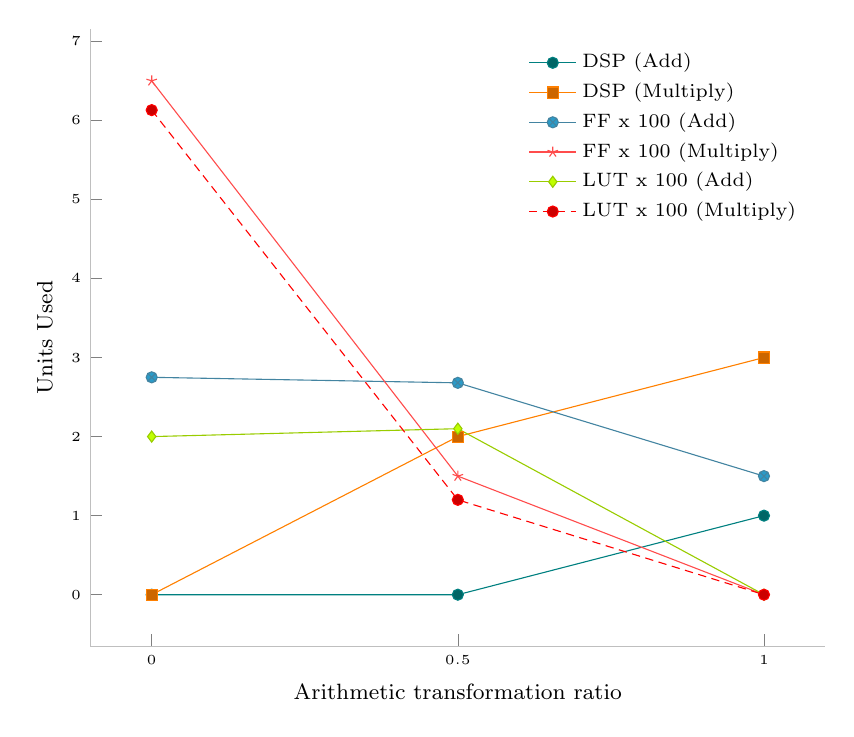
\begin{tikzpicture}
      \begin{axis}[
        cycle list name=exotic,
        xmin=0,
        ymin=0,
        axis y line*=left,
        axis x line* =bottom,
        xlabel=Arithmetic transformation ratio,
        ylabel=Units Used,
        xtick={0, 0.5, 1},
        legend columns=1,
        legend entries={
          DSP (Add),
          DSP (Multiply),
          FF x 100 (Add),
          FF x 100 (Multiply),
          LUT x 100 (Add),
          LUT x 100 (Multiply),
        },
        legend style={
          draw=none,
          cells={anchor=west}
        }
        ]
        \addplot coordinates {
          (0, 0)
          (0.5, 0)
          (1, 1)
        };
        \addplot coordinates {
          (0, 0)
          (0.5, 2)
          (1, 3)
        };
        \addplot coordinates {
          (0, 2.75)
          (0.5, 2.68)
          (1, 1.50)
        };
        \addplot coordinates {
          (0, 6.5)
          (0.5, 1.5)
          (1, 0)
        };
        \addplot coordinates {
          (0, 2)
          (0.5, 2.1)
          (1, 0)
        };
        \addplot coordinates {
          (0, 6.13)
          (0.5, 1.2)
          (1, 0)
        };
      \end{axis}
    \end{tikzpicture}
  \end{figure}
\end{frame}

\begin{frame}{Evaluation: RTM Word Length Exploration}
  \begin{figure}
    \centering
    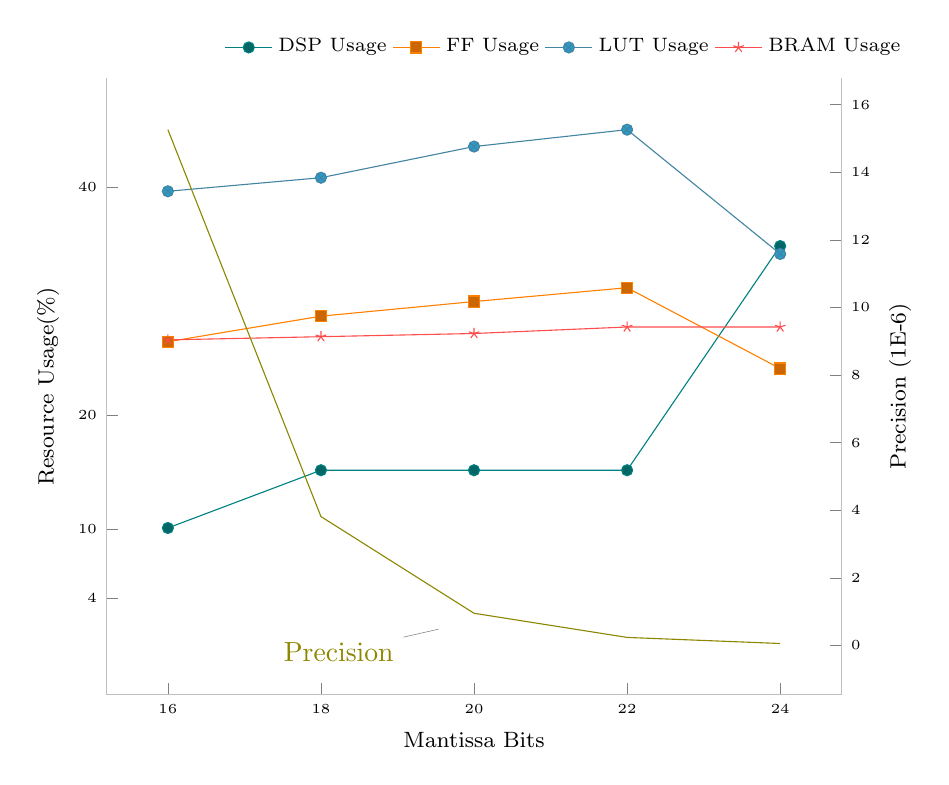
\begin{tikzpicture}
      \begin{axis}[
        cycle list name=exotic,
        ymin=0,
        axis y line*=left,
        axis x line*=bottom,
        xlabel=Mantissa Bits,
        ylabel=Resource Usage(\%),
        xtick=data,
        ytick={4, 10, 20, 40, 50, 70, 80, 100},
        legend columns=4,
        legend entries={
          DSP Usage,
          FF Usage,
          LUT Usage,
          BRAM Usage},
        legend style={
          draw=none,
          anchor=east,
          at={(1.1, 1.05)}
        }
        ]
        \addplot coordinates {
          (24, 34.82)
          (22, 15.18)
          (20, 15.18)
          (18, 15.18)
          (16, 10.12)
        };
        \addplot coordinates {
          (24, 24.09)
          (22, 31.17)
          (20, 29.96)
          (18, 28.68)
          (16, 26.44)
        };
        \addplot coordinates {
          (24, 34.13)
          (22, 45.02)
          (20, 43.54)
          (18, 40.81)
          (16, 39.62)
        };
        \addplot coordinates {
          (24, 27.73)
          (22, 27.73)
          (20, 27.16)
          (18, 26.88)
          (16, 26.60)
        };
      \end{axis}
      \begin{axis}[
        ylabel=Precision (1E-6),
        axis y line*=right,
        axis x line=none,
        ]
        \addplot[color=olive] coordinates {
          (16, 15.2585)
          (18, 3.8146)
          (20, 0.9536)
          (22, 0.2394)
          (24, 0.0596)
        } node [pos=0.8,pin={190:Precision},inner sep=20pt] {};
      \end{axis}
    \end{tikzpicture}
  \end{figure}
\end{frame}

\begin{frame}{Evaluation: RTM Parallelism}
  \begin{figure}[!h]
    \centering
    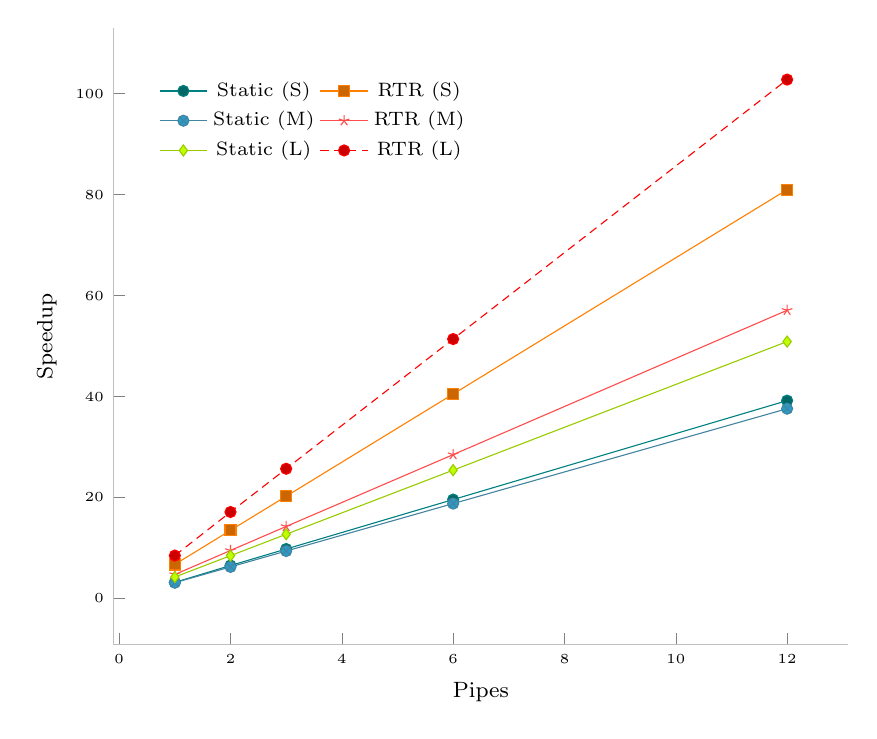
\begin{tikzpicture}
      \begin{axis}[
        cycle list name=exotic,
        xmin=1,
        ymin=1,
        xlabel=Pipes,
        ylabel=Speedup,
        axis x line* =bottom,
        axis y line* = left,
        legend columns=2,
        legend entries={
          Static (S),
          RTR (S),
          Static (M),
          RTR (M),
          Static (L),
          RTR (L)},
        legend style={
          draw=none,
          at={(0.05,0.85) },
          anchor=west
        }
        ]
        \addplot coordinates {
          (1, 3.2)
          (2, 6.53)
          (3, 9.8)
          (6, 19.6)
          (12, 39.2)
        };
        \addplot coordinates {
          (1, 6.75)
          (2, 13.5)
          (3, 20.25)
          (6, 40.5)
          (12, 81)
        };
        \addplot coordinates {
          (1, 3.13)
          (2, 6.26)
          (3, 9.4)
          (6, 18.8)
          (12, 37.6)
        };
        \addplot coordinates {
          (1, 4.75)
          (2, 9.51)
          (3, 14.27)
          (6, 28.5)
          (12, 57.1)
        };
        \addplot coordinates {
          (1, 4.25)
          (2, 8.48)
          (3, 12.725)
          (6, 25.42)
          (12, 50.9)
        };
        \addplot coordinates {
          (1, 8.5)
          (2, 17.13)
          (3, 25.7)
          (6, 51.4)
          (12, 102.8)
        };
      \end{axis}
    \end{tikzpicture}
  \end{figure}



\end{frame}


\begin{frame}{Evaluation: Benchmark}
  Comparing manual MaxCompiler designs to FAST designs:
  \begin{table}
    \renewcommand{\arraystretch}{1.2}
    \begin{tabular}{l|p{1cm}|p{1cm}|c|p{2cm}}
      \textbf{Kernel} & \textbf{LOC} & \textbf{API Calls} & \textbf{Performance}              & \textbf{Resource}
      \\
      \hline\hline
      CmdRead         & 1.76               & 4.33                     & \multirow{2}{*}{$ > 75\%$}        & \multirow{6}{3cm}{$\approx 100\%$} \\
      CmdWrite        & 1.45               & 4.13                     &                                   &                              \\
      \cline{1-4}
      RTM             & 1.17               & 10                       & \multirow{5}{*}{$ \approx 100\%$} &                              \\
      SGSmooth        & 1.85               & 14                       &                                   &                              \\
      SGDifff         & 1.75               & 14                       &                                   &                              \\
      Black-Scholes   & 2.51               & 5.5                      &                                   &                              \\
      \cline{5-5}
      Add Prediction  & 1.67               & 16                       &                                   &    $ \approx 123 \% $                          \\
    \end{tabular}
  \end{table}

\end{frame}
\section{Conclusions}

\begin{frame}{Current and Future Work}

  \begin{itemize}
  \setlength{\itemsep}{10pt}

  \item Finish second paper for FPT'13: aspect descriptions and tools
    for run-time reconfiguration

  \item Cover other classes of parallel computation

  \item Cover heterogeneous systems

  \item Support other frontend languages

  \item Cover other applications domains

  \item Improved run-time support (CPU -- DFE interface)

  \item Automated translation to dataflow designs

  \item Validate improved productivity and
    portability claims

  \end{itemize}
\end{frame}


\begin{frame}{Summary}

  \begin{beamerboxesrounded}{Aspect-driven Approach}
    \begin{itemize}
    \item improve productivity by encapsulating optimisations
    \item improve efficiency by effective design space exploration
    \end{itemize}
  \end{beamerboxesrounded}

  \begin{beamerboxesrounded}{FAST Dataflow Language}
    \begin{itemize}
    \item simple, intuitive specification of dataflow designs
    \item integrate AOP techniques with dataflow compilation tools
    \end{itemize}
  \end{beamerboxesrounded}

  \begin{beamerboxesrounded}{Aspect Descriptions}
    \begin{itemize}
      \item improve performance, productivity; automate exploration
      \item support for run-time reconfiguration
    \end{itemize}
  \end{beamerboxesrounded}

  \begin{beamerboxesrounded}{Demonstrate Automated Design Flow}
    \begin{itemize}
    \item produced fastest most energy efficient  RTM dataflow design
    \item 40-80\% code reduction, 4 -- 16 times less API calls
    \item best paper candidate at ASAP 2013 (4 of 125 submissions)
    \end{itemize}
  \end{beamerboxesrounded}

\end{frame}


\begin{frame}{References}
  {\footnotesize
  \begin{thebibliography}{1}
  \bibitem{himeno} Phillips, Everett H., and Massimiliano
    Fatica. \emph{Implementing the Himeno benchmark with CUDA on GPU
    clusters.} Parallel \& Distributed Processing (IPDPS), 2010 IEEE
    International Symposium on. IEEE, 2010.
  \bibitem{datta} Datta, Kaushik, et al. \emph{Stencil computation
      optimization and auto-tuning on state-of-the-art multicore
      architectures.} Proceedings of the 2008 ACM/IEEE conference on
    Supercomputing. IEEE Press, 2008.
  \bibitem{cirque}Yang, Yang, et al. \emph{A hybrid circular queue method
    for iterative stencil computations on GPUs.} Journal of Computer
    Science and Technology 27.1 (2012): 57-74.
  \bibitem{arraya} Araya-Polo, Mauricio, et al. \emph{Assessing
      accelerator-based HPC reverse time migration.} Parallel and
    Distributed Systems, IEEE Transactions on 22.1 (2011): 147-162.
  \bibitem{xinyu} Niu, Xinyu, et al. \emph{Exploiting run-time
    reconfiguration in stencil computation.} Field Programmable Logic
    and Applications (FPL), 2012 22nd International Conference
    on. IEEE, 2012.
  \end{thebibliography}
  }

\end{frame}

\end{document}
